%Calaway;section 9; page 148; Max-Min Story Problem Technique
%Calaway;section 9; page 149; Example 1
%Calaway;section 9; page 149; Example 2 and %question 8 from https://www.math.tamu.edu/~mayaj/m142_Chapter5_Sec5.6completed.pdf
%Dave's handout 2.2 2nd derivative rule
%Calaway;section 9; MR=MC
\vspace{-0.25 in}
\begin{framed}
\subsection*{Objectives}
\begin{itemize}
    \item Set up an objective equation and an constraint equation from real-world problems.
    \item Use calculus to find optimal values from the objective question and constraint equation in the context of real-world problems.
\end{itemize}

%%%Reading Assignment%%%
\subsection*{Suggested Reading:}
\begin{itemize}
\item \cite{Calaway}\footnotemark[1]
   \begin{itemize}
        \item \emph{Section 2.9 Applied Optimization}
    \end{itemize}

\item \cite{openstax}\footnotemark[2]\textsuperscript{,}\footnotemark[3]
    \begin{itemize}
        \item \emph{Section 4.7 Applied Optimization Problems}
    \end{itemize}

\end{itemize}
%\subsection*{Supplemental Materials:}
%%%Key Terms%%%
\subsection*{Key Terms and Concepts:} 

\begin{multicols}{2}
\begin{itemize}
    \item Objective Equation
    \item Constraint Equation
    
\end{itemize}
\end{multicols}
\end{framed}
\footnotetext[1]{Available free to download from \url{http://www.opentextbookstore.com/details.php?id=14} .}
\footnotetext[2]{Available free to download from \url{https://openstax.org/details/books/calculus-volume-1} .}
\footnotetext[3]{Disregard any examples with trigonometry.}

\newpage
%%%%%%%%%%START LESSON CONTENT%%%%%%%%%%%%%
%\noindent\makebox[\linewidth]{\rule{\textwidth}{0.8pt}}
\Opensolutionfile{ans}[ans9]
\Opensolutionfile{ansL}[ansL9]
%%%%%%%%%%%%%%%%Start First Topic%%%%%%%%%%%%%%%%%%%%%%%%%%%%%
\subsection*{Objective Function:}
The process of finding \underline{maxima or minima} is called optimization. The function we are optimizing is called the \textbf{objective function}. The objective function can be recognized by its proximity to “est” words (greatest, least, highest, farthest, most, …)

\subsection*{Types of Optimization Problems:}

There are two main types of applied optimization problems: \emph{Unconstrained Optimization} and \emph{Constrained Optimization}.

\subsection*{Unconstrained Optimization}
An unconstrained optimization problem is  a problem where an \textbf{objective function} is being optimized (minimized or maximized) and none of the variable(s) in the objective function are constrained.

\begin{tcolorbox}[title={Solving \textbf{Unconstrained} Optimization Problems: Problem-Solving Strategy}]
\begin{enumerate}[leftmargin=*]
\item Identify the unknown variable for which you are solving.  
\item Determine which \textbf{quantity is to be maximized or minimized}.
    \begin{itemize}
        \item Write a formula \textbf{(objective equation)} for the quantity to be maximized or minimized in terms of the unknown variable. 
    \end{itemize}
\item Find critical value(s) using the first derivative test for local extremum (extrema).
    \renewcommand{\labelenumii}{(\roman{enumii})}
    \begin{enumerate}
        \item Determine the first derivative of the objective function from the previous step. 
        \item Set the first derivative function equal to zero and then solve for the unknown variable.
    \end{enumerate}
    \renewcommand{\labelenumi}{\arabic{enumi}}
\item Using either the first derivative test or the seoncd derivative test, determine if the local extremum (extrema) is (are) local maximum or local minimum. 
\item Look back at the question to make sure you answered what was asked. \textbf{Translate your number} answer back into English.
\renewcommand{\labelenumi}{(\alph{enumi})}
    \begin{enumerate}
        \item If required, use the \underline{objective function} to find the maximum/minimum value . 
    \end{enumerate}
\end{enumerate}
\end{tcolorbox}
%%%Exercise 18 from Calaway; 2.9; pg. 156%%%
\begin{example}
The total cost in dollars for Alicia to make $\bm{q}$ oven mitts is given by $\bm{C(q)=0.01q^2+1.5q+64}$.
\renewcommand{\labelenumi}{(\alph{enumi})}
\begin{enumerate}[leftmargin=*]
    \item Find a function that gives the \textbf{average cost}.\\
    	\begin{displaymath}
		\begin{split}
		\textbf{SOLUTION:} \quad	\textbf{Average Cost:}\quad AC(q) &=\frac{C(q)}{q}=\frac{0.01q^2+1.5q+64}{q}\\
			                                  &=\frac{0.01q^2}{q}+\frac{1.5q}{q}+\frac{64}{q}\\
			                                  &=0.01q+1.5+\frac{64}{q}
		\end{split}
	\end{displaymath}
	\newpage
    \item Find the quantity that \underline{minimizes} the \textbf{average cost}.
    \vspace*{6in}
    \item Find a function that gives the \textbf{marginal cost}.\\
    	\begin{displaymath}
		\begin{split}
		\textbf{SOLUTION:} \quad \textbf{Total Cost:}\quad C(q) &=0.01q^2+1.5q+64\\
			\textbf{Marginal Cost:}\quad C'(q) &=0.02q+1.5\\
		\end{split}
	\end{displaymath}
    \item Confirm that the \underline{average cost and marginal cost are equal} at your answer to part (b).\\
    
    	\begin{displaymath}
		\begin{split}
	\textbf{SOLUTION:} \quad	AC(q) &=C'(q)\\
	   0.01q+1.5+\frac{64}{q} &=0.02q+1.5\\
	   q&=80 \quad \text{oven mitts}
		\end{split}
	\end{displaymath}
\end{enumerate}
    %%short answer
    \begin{sol}
    \onehalfspacing{
    \begin{enumInline1}
    \item $AC(q)=0.01q+1.5+\frac{64}{q}$
    \item $q_{min}=$ 80 oven mitts
    \item $MC(q)=C'(q)=0.02q+1.5 $
    \item $AC(q)=C'(q)\Longrightarrow q=$ 80 oven mitts
    \end{enumInline1} }
    
    \end{sol}
    %%solution
    \begin{solL}
    Complete solution here.....
    
    \end{solL}
    
\end{example}

\vspace*{\stretch{1}}
%%%%%%%%%%%%%%%%%%%%%%%%%%%%%%%%%%%%%%%%%%%%%%
\begin{tcolorbox}
Average Cost has critical points when Average Cost and Marginal Cost are equal.
\end{tcolorbox}

\newpage
%%%Example 4 from Calaway; 2.9; pg. 152%%%
\begin{example}
A company sells $\bm q$ ribbon winders per year at \$ $\bf{p}$ per ribbon winder. The demand function for ribbon winders is given by: $\bf{p=300-0.02q}$. The ribbon winders cost \$30 apiece to manufacture, plus there are fixed costs of \$9000 per year. \textbf{Find the quantity} where profit is maximized.
\renewcommand{\labelenumi}{(\alph{enumi})}
\begin{enumerate}[leftmargin=*]
    \item Find a function that gives the \textbf{revenue} with the quantity ($q$).\\
    	\begin{displaymath}
		\begin{split}
		\textbf{SOLUTION:} \quad	\textbf{Revenue:}\quad R(q) &=q\cdot p(q)=q\cdot (300-0.02q)=300q-0.02q^2
		\end{split}
	\end{displaymath}
    \item Find a function that gives the \textbf{cost} with the quantity ($q$).\\
    	\begin{displaymath}
		\begin{split}
		\textbf{SOLUTION:} \quad	\textbf{Total Cost}:\quad C(q) &=30\cdot q+9000
		\end{split}
	\end{displaymath}
    \item Find a function that gives the \textbf{profit} with the quantity ($q$).\\
    	\begin{displaymath}
		\begin{split}
		\textbf{SOLUTION:} \quad \textbf{Profit}:\quad P(q) &=R(q)-C(q)\\
			                           &=(300q-0.02q^2)-(30\cdot q+9000)=-0.02q^2+270q-9000\\
		\end{split}
	\end{displaymath}
    \item Find the \textbf{quantity} that \underline{maximizes} the profit.
    
    \newpage
    \item Find a function that gives the \textbf{marginal revenue}.\\
    	\begin{displaymath}
		\begin{split}
		\textbf{SOLUTION:} \quad \textbf{Revenue:}\quad R(q) &=300q-0.02q^2\\
			\textbf{Marginal Revenue:}\quad R'(q) &=300-0.04q\\
		\end{split}
	\end{displaymath}
	
    \item Find a function that gives the \textbf{marginal cost}.\\
    	\begin{displaymath}
		\begin{split}
		\textbf{SOLUTION:} \quad \textbf{Total Cost:}\quad C(q) &=30\cdot q+9000\\
			\textbf{Marginal Cost:}\quad C'(q) &=30\\
		\end{split}
	\end{displaymath}
    \item Confirm that the \underline{marginal revenue and marginal cost} are equal at your answer to (d).\\
    	\begin{displaymath}
		\begin{split}
	\textbf{SOLUTION:} \quad	R'(q) &=C'(q)\\
	   300-0.04q &=30\\
	   q&=6,750 \quad \text{ribbon winders}
		\end{split}
	\end{displaymath}
\end{enumerate}
    %%short answer
    \begin{sol}
    \onehalfspacing{
    \begin{enumInline1}
    \item $R(q)=300q-0.02q^2$
    \item $C(q)=9000+30q$ \hspace{0.25cm}
    \item $P(q)=-0.02q^2+270q-9000$
    \item $q_{max}=$6,750 ribbon winders 
    \item $MR(q)=300-0.04q$ 
    \item  $MC=30$ \hspace{\fill}
    \item  $R'(q)=C'(q)\Longrightarrow q=$ 6,750 ribbon winders 
    \end{enumInline1}
    }
    
    \end{sol}
    %%solution
    \begin{solL}
    Complete solution here.....
    
    \end{solL}
    
\end{example}

%%%%%%%%%%%%%%%%%%%%%%%%%%%%%%%%%%%%%%%%%%%
\begin{tcolorbox}
Profit has critical points when Marginal Revenue and Marginal Cost are equal.
\end{tcolorbox}

\begin{figure}[H]
		\flushleft
		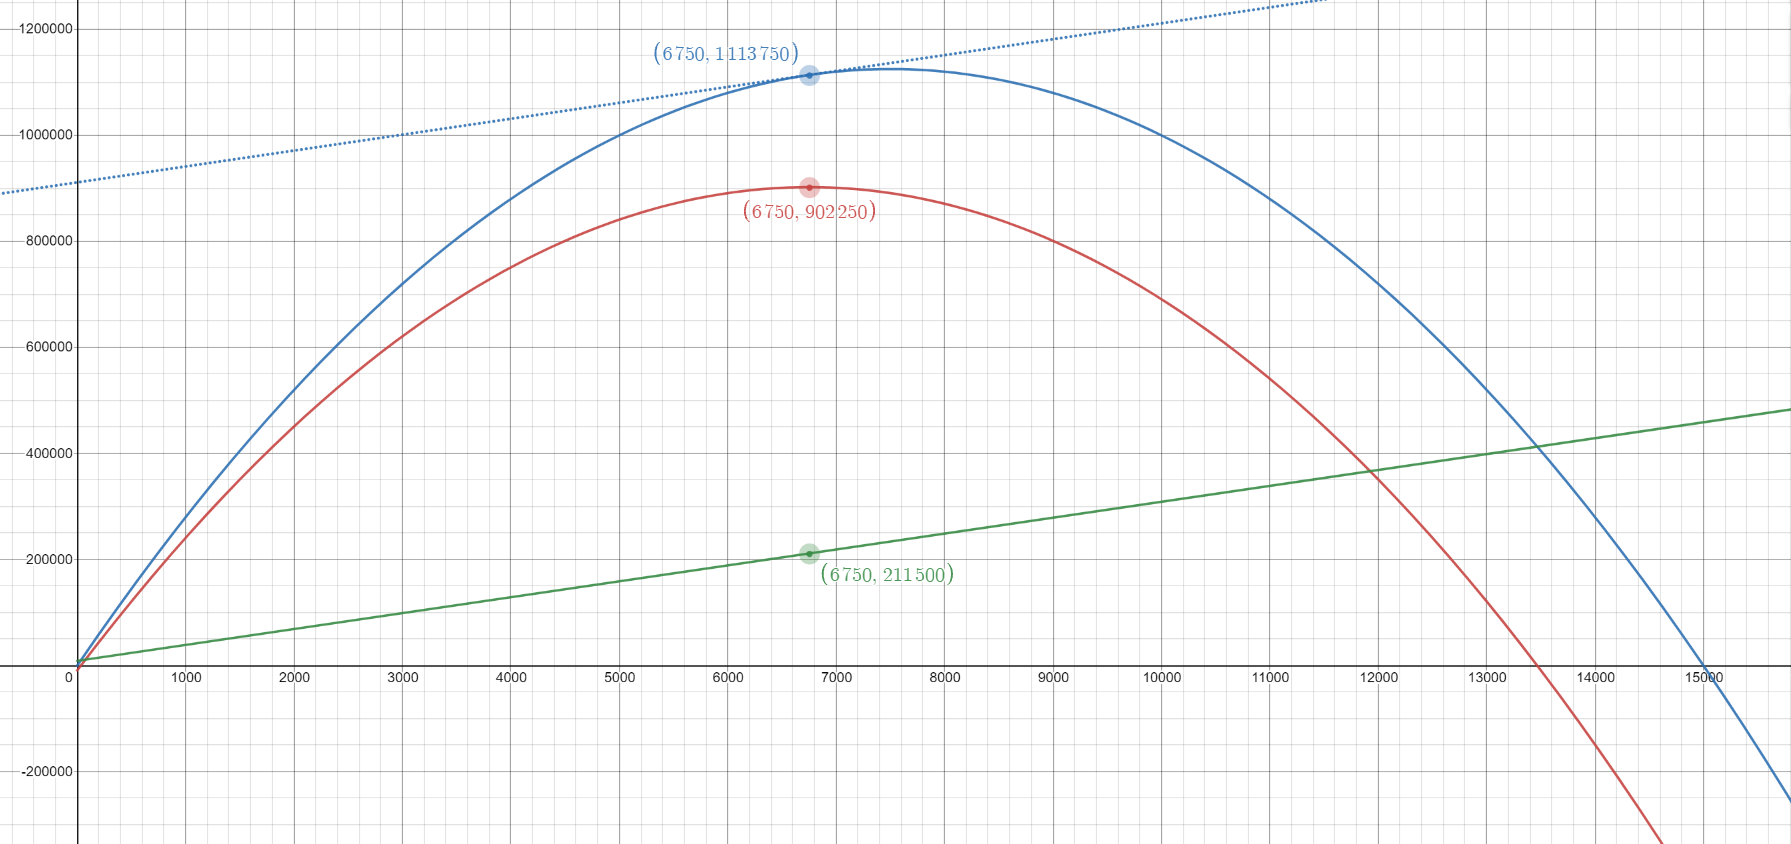
\includegraphics[scale=0.55]{images/appliedOptimization/Optimization_maxRev1.PNG}
		%\caption{}
		\label{fig:fencing1}
	\end{figure}
	
\begin{figure}[H]
		\flushleft
		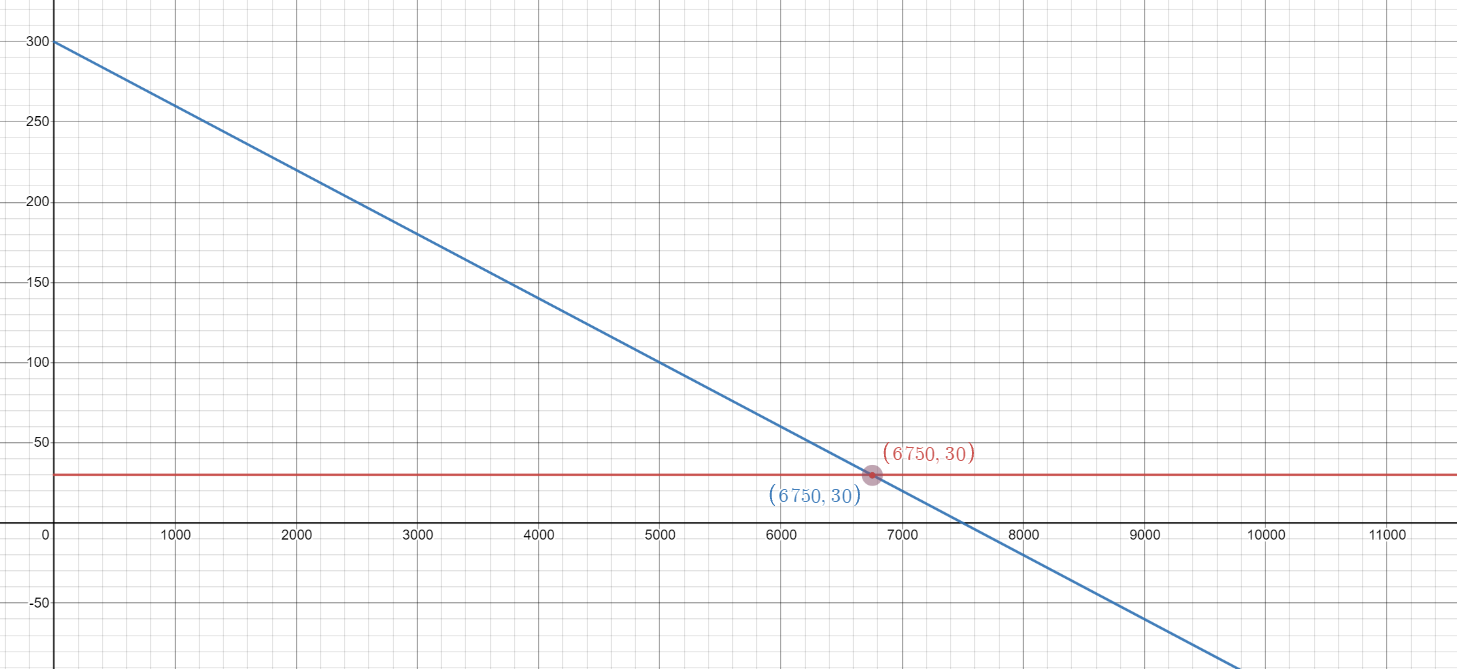
\includegraphics[scale=0.5]{images/appliedOptimization/Optimization_maxRev2.PNG}
		%\caption{}
		\label{fig:fencing1}
	\end{figure}
\newpage
\subsection*{Constrained Optimization}
\noindent Like many concepts and techniques that you have been exposed to in math classes, derivatives also have importance in applied problems. We will consider examples of a certain type of application known as "constrained optimization" problems. The common theme in these problems is that we will determine a function that we hope to maximize or minimize subject to a constraint that does not allow us to make the value of the function arbitrarily large or small.

\subsection*{Constraint Equation:}
In many cases, there are two (or more) variables in the problem. If there is an equation that \underline{relates the variables} we can solve for one of them in terms of the others, and write the objective function as a function of just one variable. Equations that relate the variables in this way are called \textbf{constraint equations}. Include the appropriate units.
\vspace{0.5 cm}

%%%%%%%%%%%%%%%openstax: Calculus Volume 1; 4.7 applied Optimization Problems%%%%%%%%%%%
\begin{tcolorbox}[title={Solving \textbf{Constrained} Optimization Problems: Problem-Solving Strategy}]
\begin{enumerate}[leftmargin=*]
\item Identify all unknown variables for which you are solving.  If applicable, draw a figure and label all variables.
\item Determine which \textbf{quantity is to be maximized or minimized}.
    \begin{itemize}
        \item Write a formula \textbf{(objective equation)} for the quantity to be maximized or minimized in terms of the unknown variables. 
    \end{itemize}
\item Determine which \textbf{quantity is to be fixed}
    \begin{itemize}
        \item Write any equations \textbf{(constraint equations)} relating the unknown variables in the objective function.  
    \end{itemize}
\item Solve the constraint equation for one variable and substitute into the objective function. Now you have \textbf{the objective equation of one variable}.
\item Find critical value(s) using the first derivative test for local extremum (extrema).
    \renewcommand{\labelenumii}{(\roman{enumii})}
    \begin{enumerate}
        \item Determine the first derivative of the objective function with one variable (from the previous step). 
        \item Set the first derivative function equal to zero and then solve for the unknown variable.
    \end{enumerate}
    \renewcommand{\labelenumi}{\arabic{enumi}}
\item Using either the first derivative test or the seoncd derivative test, determine if the local extremum (extrema) is (are) local maximum or local minimum. 
\item Look back at the question to make sure you answered what was asked. \textbf{Translate your number} answer back into English.
\renewcommand{\labelenumi}{(\alph{enumi})}
    \begin{enumerate}
        \item If required, use the \underline{constraint equation(s)} to solve for the other unknown variable(s). 
        \item If required, use the \underline{objective function} to find the maximum/minimum value . 
    \end{enumerate}
\end{enumerate}
\end{tcolorbox}
\newpage
%%%%%%%%%%%%%Question 1 from https://www.math.tamu.edu/~mayaj/m142_Chapter5_Sec5.6completed.pdf
\begin{example}
\textbf{Find two non-negative numbers} whose sum is 44 and whose product is a \underline{maximum}. Also, \textbf{find the maximum value} of the product of these numbers.
\begin{multicols}{2}
    \begin{minipage}{0.4\textwidth}
        \begin{figure}[H]
		\flushleft
		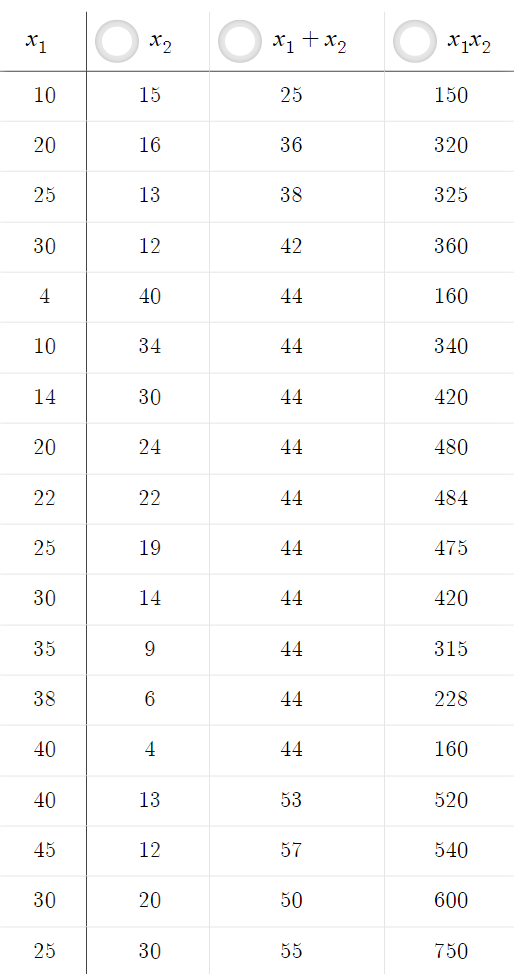
\includegraphics[scale=0.65]{images/appliedOptimization/Optimization_maxProduct2.PNG}
		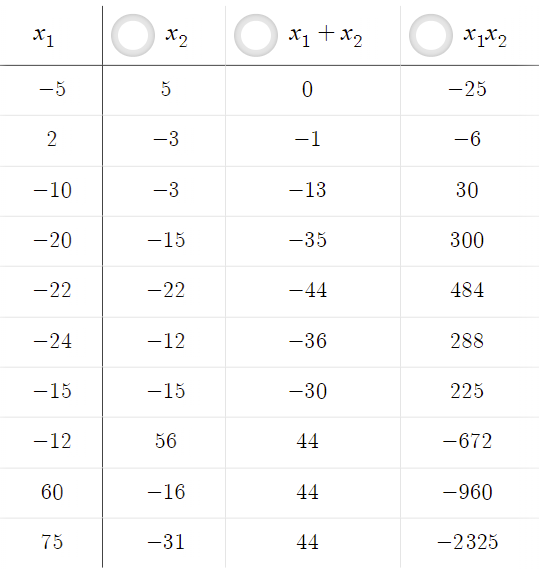
\includegraphics[scale=0.65]{images/appliedOptimization/Optimization_maxProduct1.PNG}
		%\caption{}
		\end{figure}
    \end{minipage}
    \begin{minipage}{0.6\textwidth}
    \vfill
		\begin{figure}[H]
		\centering
		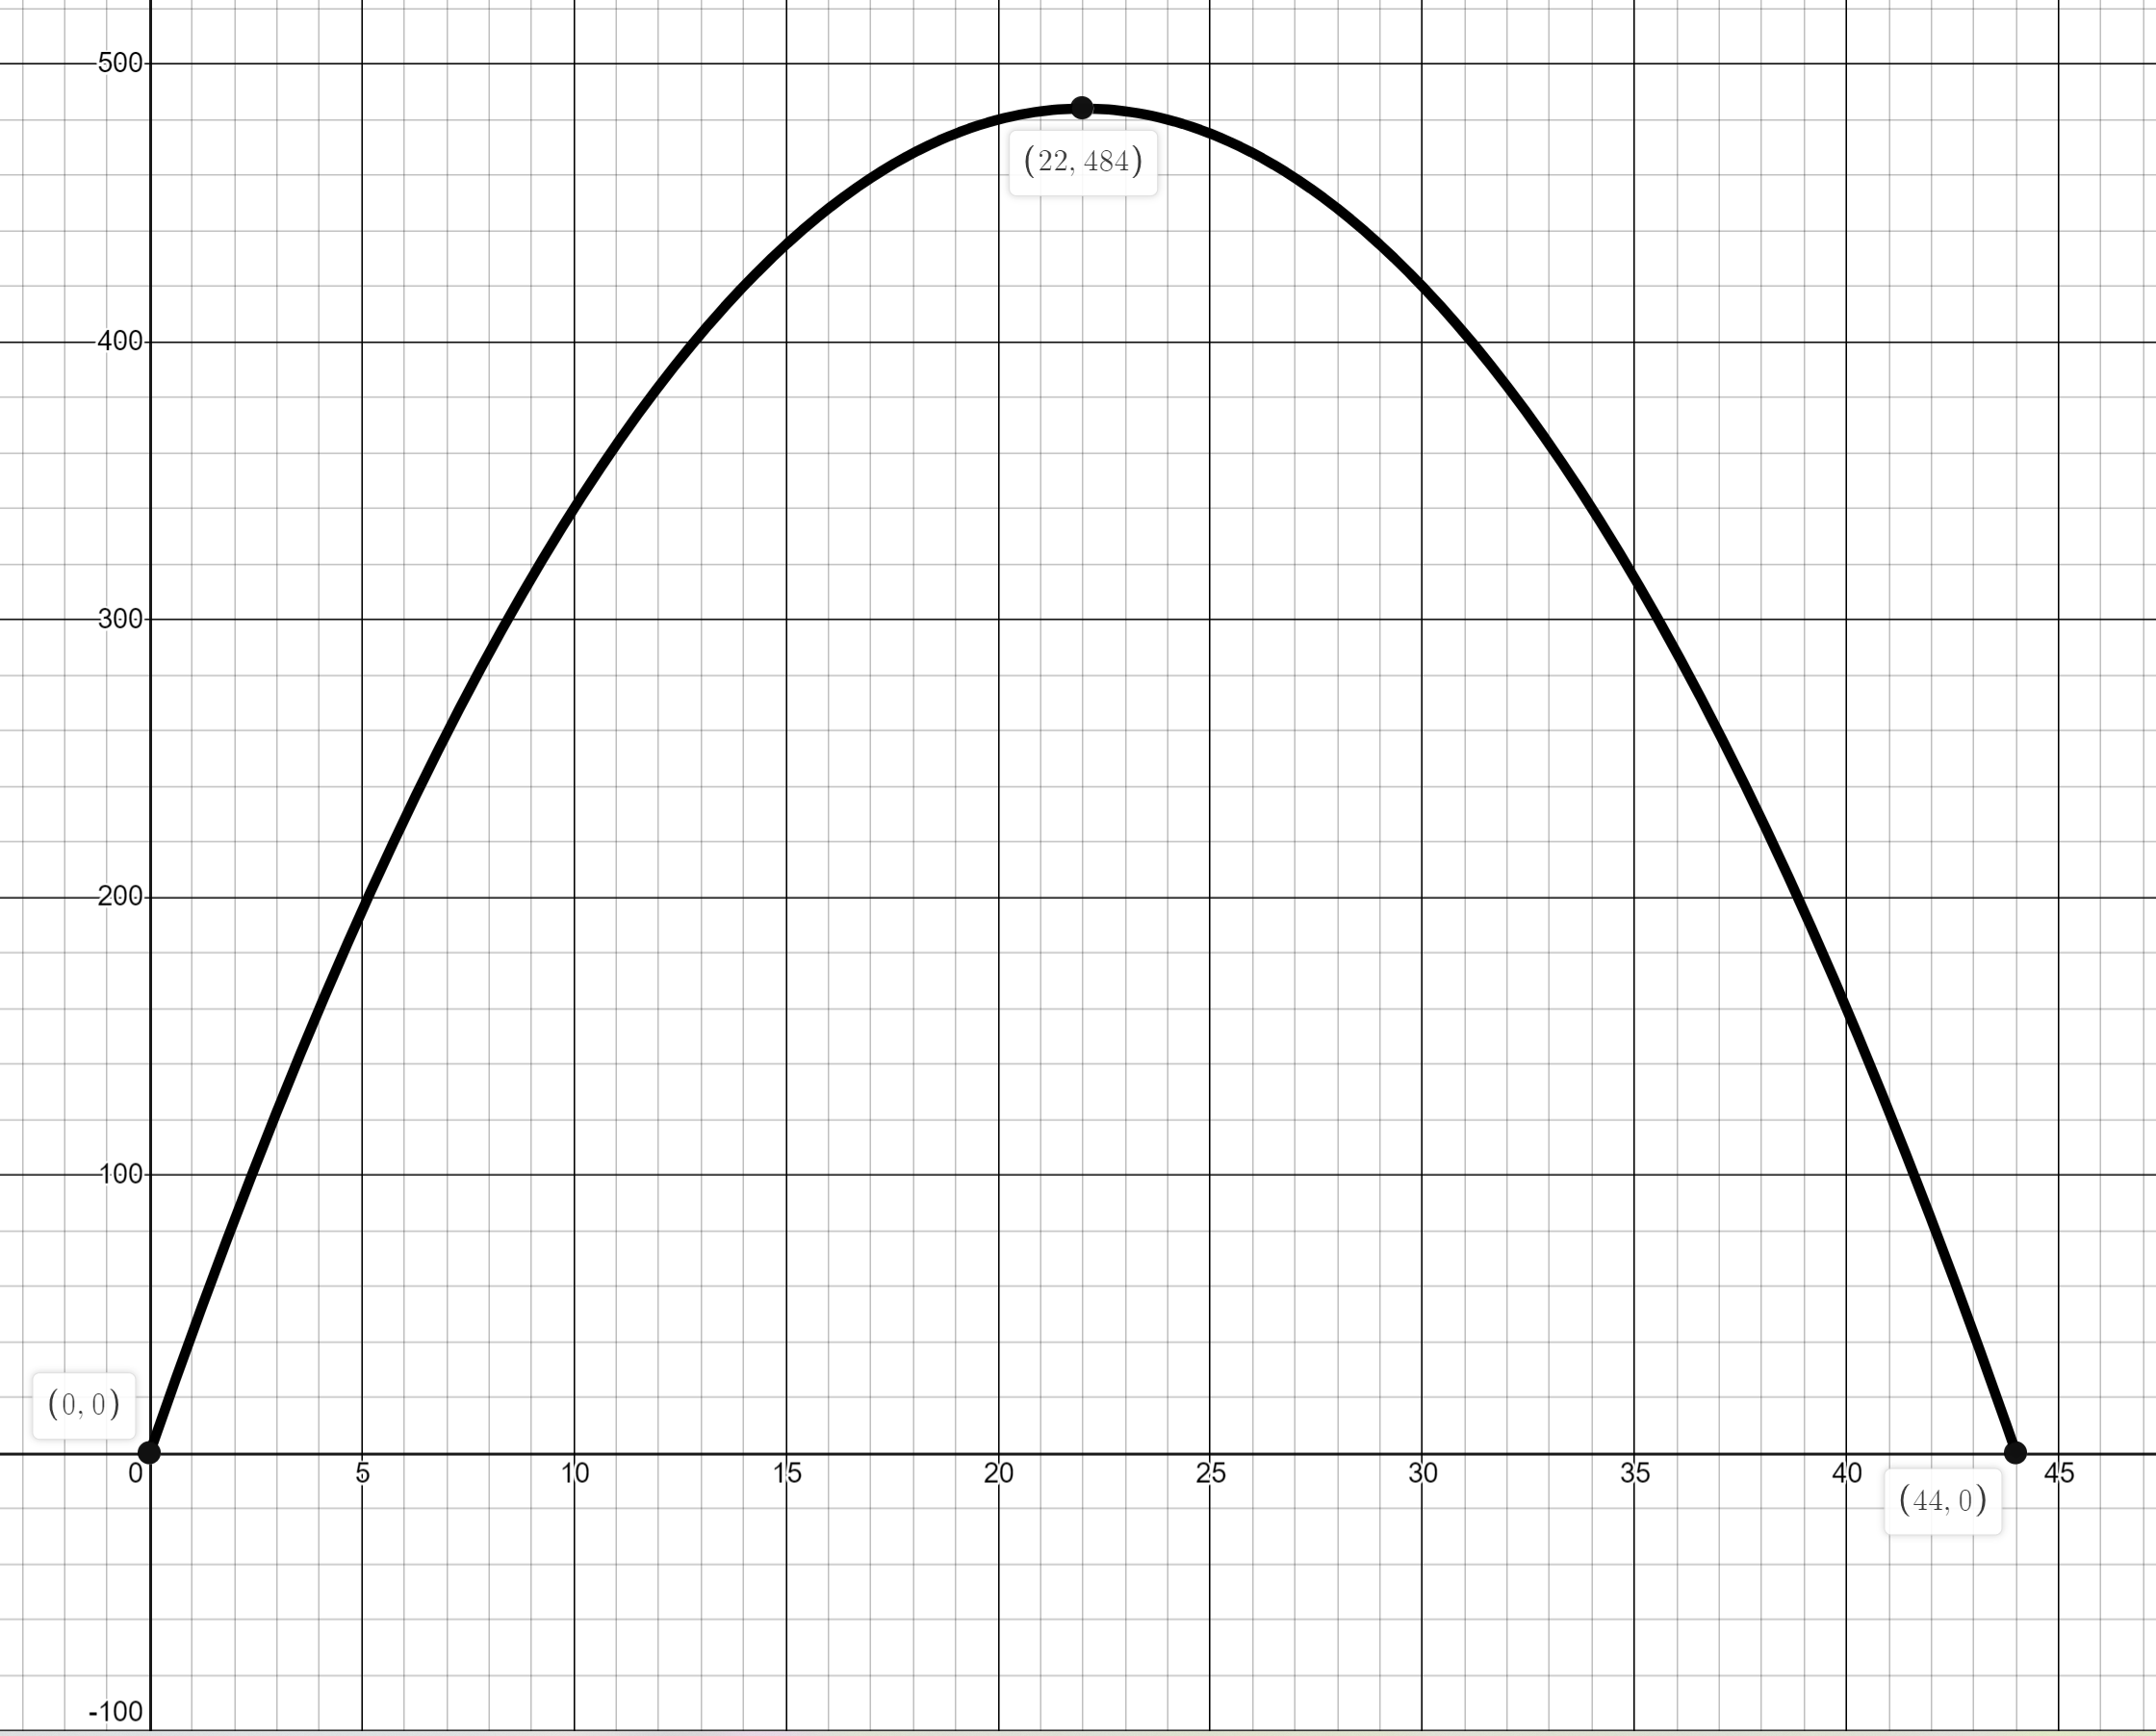
\includegraphics[scale=0.2]{images/appliedOptimization/Optimization_maxProduct3.PNG}
		%\caption{}
	    \end{figure}
    \end{minipage}
    
\end{multicols}
%%short answer
    \begin{sol}
    $x=22$; $y=22$ ; maximum value of the product: 484
    \end{sol}
    %%solution
    \begin{solL}
    Complete solution here.....
    
    \end{solL}
    
\end{example}
\newpage
%%%%%%%%%%%%%%%%%%%%%%%%%%%%%%%%%%%%%%%%%%%%%%%%%%%
%%%%%%%%%% MOM#678768 %%%%%%%
%%%%%%%%%%%%%%%%%%%%%%%%%%%%%%%%%%%%%%%%%%%%%%%%%%%%%%%
\begin{example}
%%short answer
    
     \begin{sol}
    $x=2,000$ feet; $y=3,000$ feet; Maximum area is $6,000,000$ square feet.
    \end{sol}
     
    %%solution
    \begin{solL}
    	\underline{\textbf{First Approach}}
	\begin{displaymath}
		\begin{split}
			\text{Constraint Equation:}\quad x\cdot y&=4752\\
			x&=\frac{4752}{y}\\
			\text{Objective Equation}\quad C&=48y+48x+ 48y+40x\\
			\text{Objective Equation in terms of}\quad y:\quad   C(y)&=48y+48\cdot\tb{\left(\frac{4752}{y}\right)}+ 48y+40\cdot \tb{\left(\frac{4752}{y}\right)} \\
			&=96y+88\cdot\left(\frac{4752}{y}\right)\\
			&=96y+88\cdot 4752\cdot y^{-1}\\
		\end{split}
	\end{displaymath}
	$$C'(y)=96+(-1)(88)(4752)\cdot y^{-2}$$
	
	\underline{Partition values and Critical values}
	\begin{displaymath}
		\begin{split}
			C'(y) &=0 \\
			96-(88)(4752)\cdot \frac{1}{y^{2}} &=0 \Longrightarrow 96\cdot y^2 =(88)(4752) \\
			96\cdot y^2 &=(88)(4752)\\
			y^2 &=\frac{(88)(4752)}{96}\\
			y&=\pm \sqrt{\frac{(88)(4752)}{96}}=\pm 66\\
			\text{Partition Value:}\qquad  y &= 66 \quad \text{Note: Dimensions cannot be negative.} \\
		\end{split}
	\end{displaymath}
	Since the partition value of 66 is in the domain of $f(x)$,  the partition value of $y=66$ is also the critical value. Recall that the local(relative) extremum occur only at the critical value.\\
	\underline{Sign of $A'(y)$}:\\
	
	Interval $(0,66)\quad \Longrightarrow$ \quad Test point: $y=1 \quad \Longrightarrow$ \quad $C'(1)<0$. \emph{Note that the interval starts at 0 since the width of each side of the fence cannot be negative.}\\
	Interval $(66,\infty)\quad \Longrightarrow$ \quad Test point: $y=100 \quad \Longrightarrow$ \quad $C'(100)>0$.\\
	
	\underline{Sign Chart with Critical Values}:\\
	
	\hspace*{1cm}$\bm{-}\hspace{2.25cm} \bm{+} $\\
	$\bm{0}$ -------------- $\bm{66}$  ---------------$>$\\
	
	Since the sign change from $-$ to $+$ at $y=66$,  \textbf{the local (relative) minimum (and the global (absolute) minimum) occur at} the \textbf{dimenstion} of $\bm{y=66}$ feet and $x=\frac{4752}{66}=72$ feet \\
\newline
    
    \end{solL}
    
	
\end{example}
\begin{multicols}{2}
	\begin{minipage}{0.65\textwidth}
	
\noindent Sarah is a rancher and would like to construct a corral along the north side of a river. No fencing is required along the river. The west side of the corral is adjacent to the neighbor's property, who has agreed to evenly split the cost of the fence along the west side of the corral. If Sarah would like to spend no more than \$420,000 on the project and has determined that the full cost per foot of fencing is \$70 per linear foot, determine the \textbf{dimensions} of the corral of maximum area and the \textbf{maximum area} of the corral, given the cost constraint. 	 \\
\end{minipage}

\begin{minipage}{0.55\textwidth}
	\vspace{-0.75cm}
		\begin{figure}[H]
		\flushright
		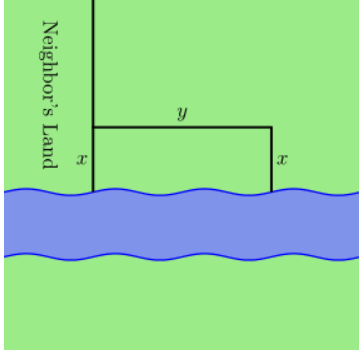
\includegraphics[scale=1.5]{images/optimization/Optimization_fencing2.PNG}
		%\caption{}
		\label{fig:fencing1}
	\end{figure}
\end{minipage}
\end{multicols}

\noindent Identify the \underline{objective equation} and the \underline{constraint equation}.
\begin{multicols}{2}
    \begin{minipage}{0.4\textwidth}
        \begin{figure}[H]
		\flushleft
		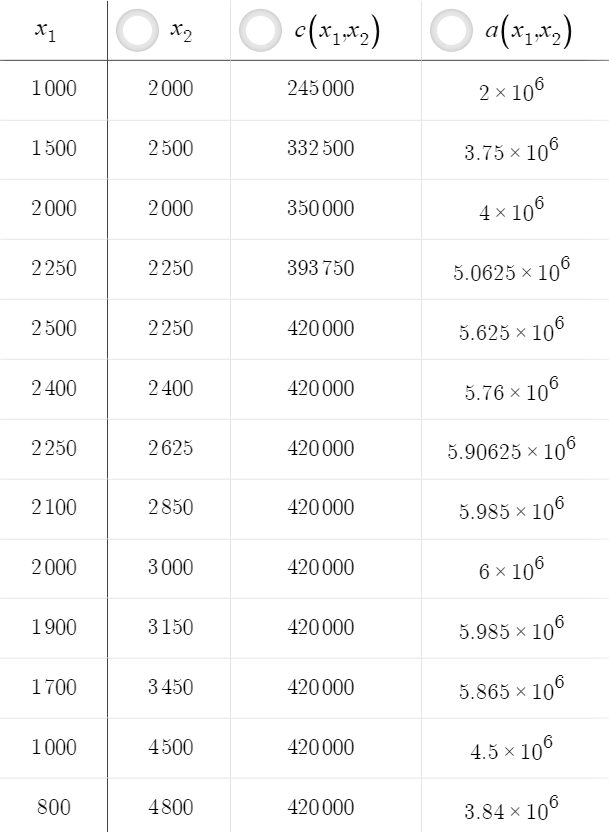
\includegraphics[scale=0.65]{images/appliedOptimization/Optimization_fencing1_ex10_4.PNG}
		%\caption{}
		\end{figure}
    \end{minipage}
    \begin{minipage}{0.6\textwidth}
    \vfill
		\begin{figure}[H]
		\centering
		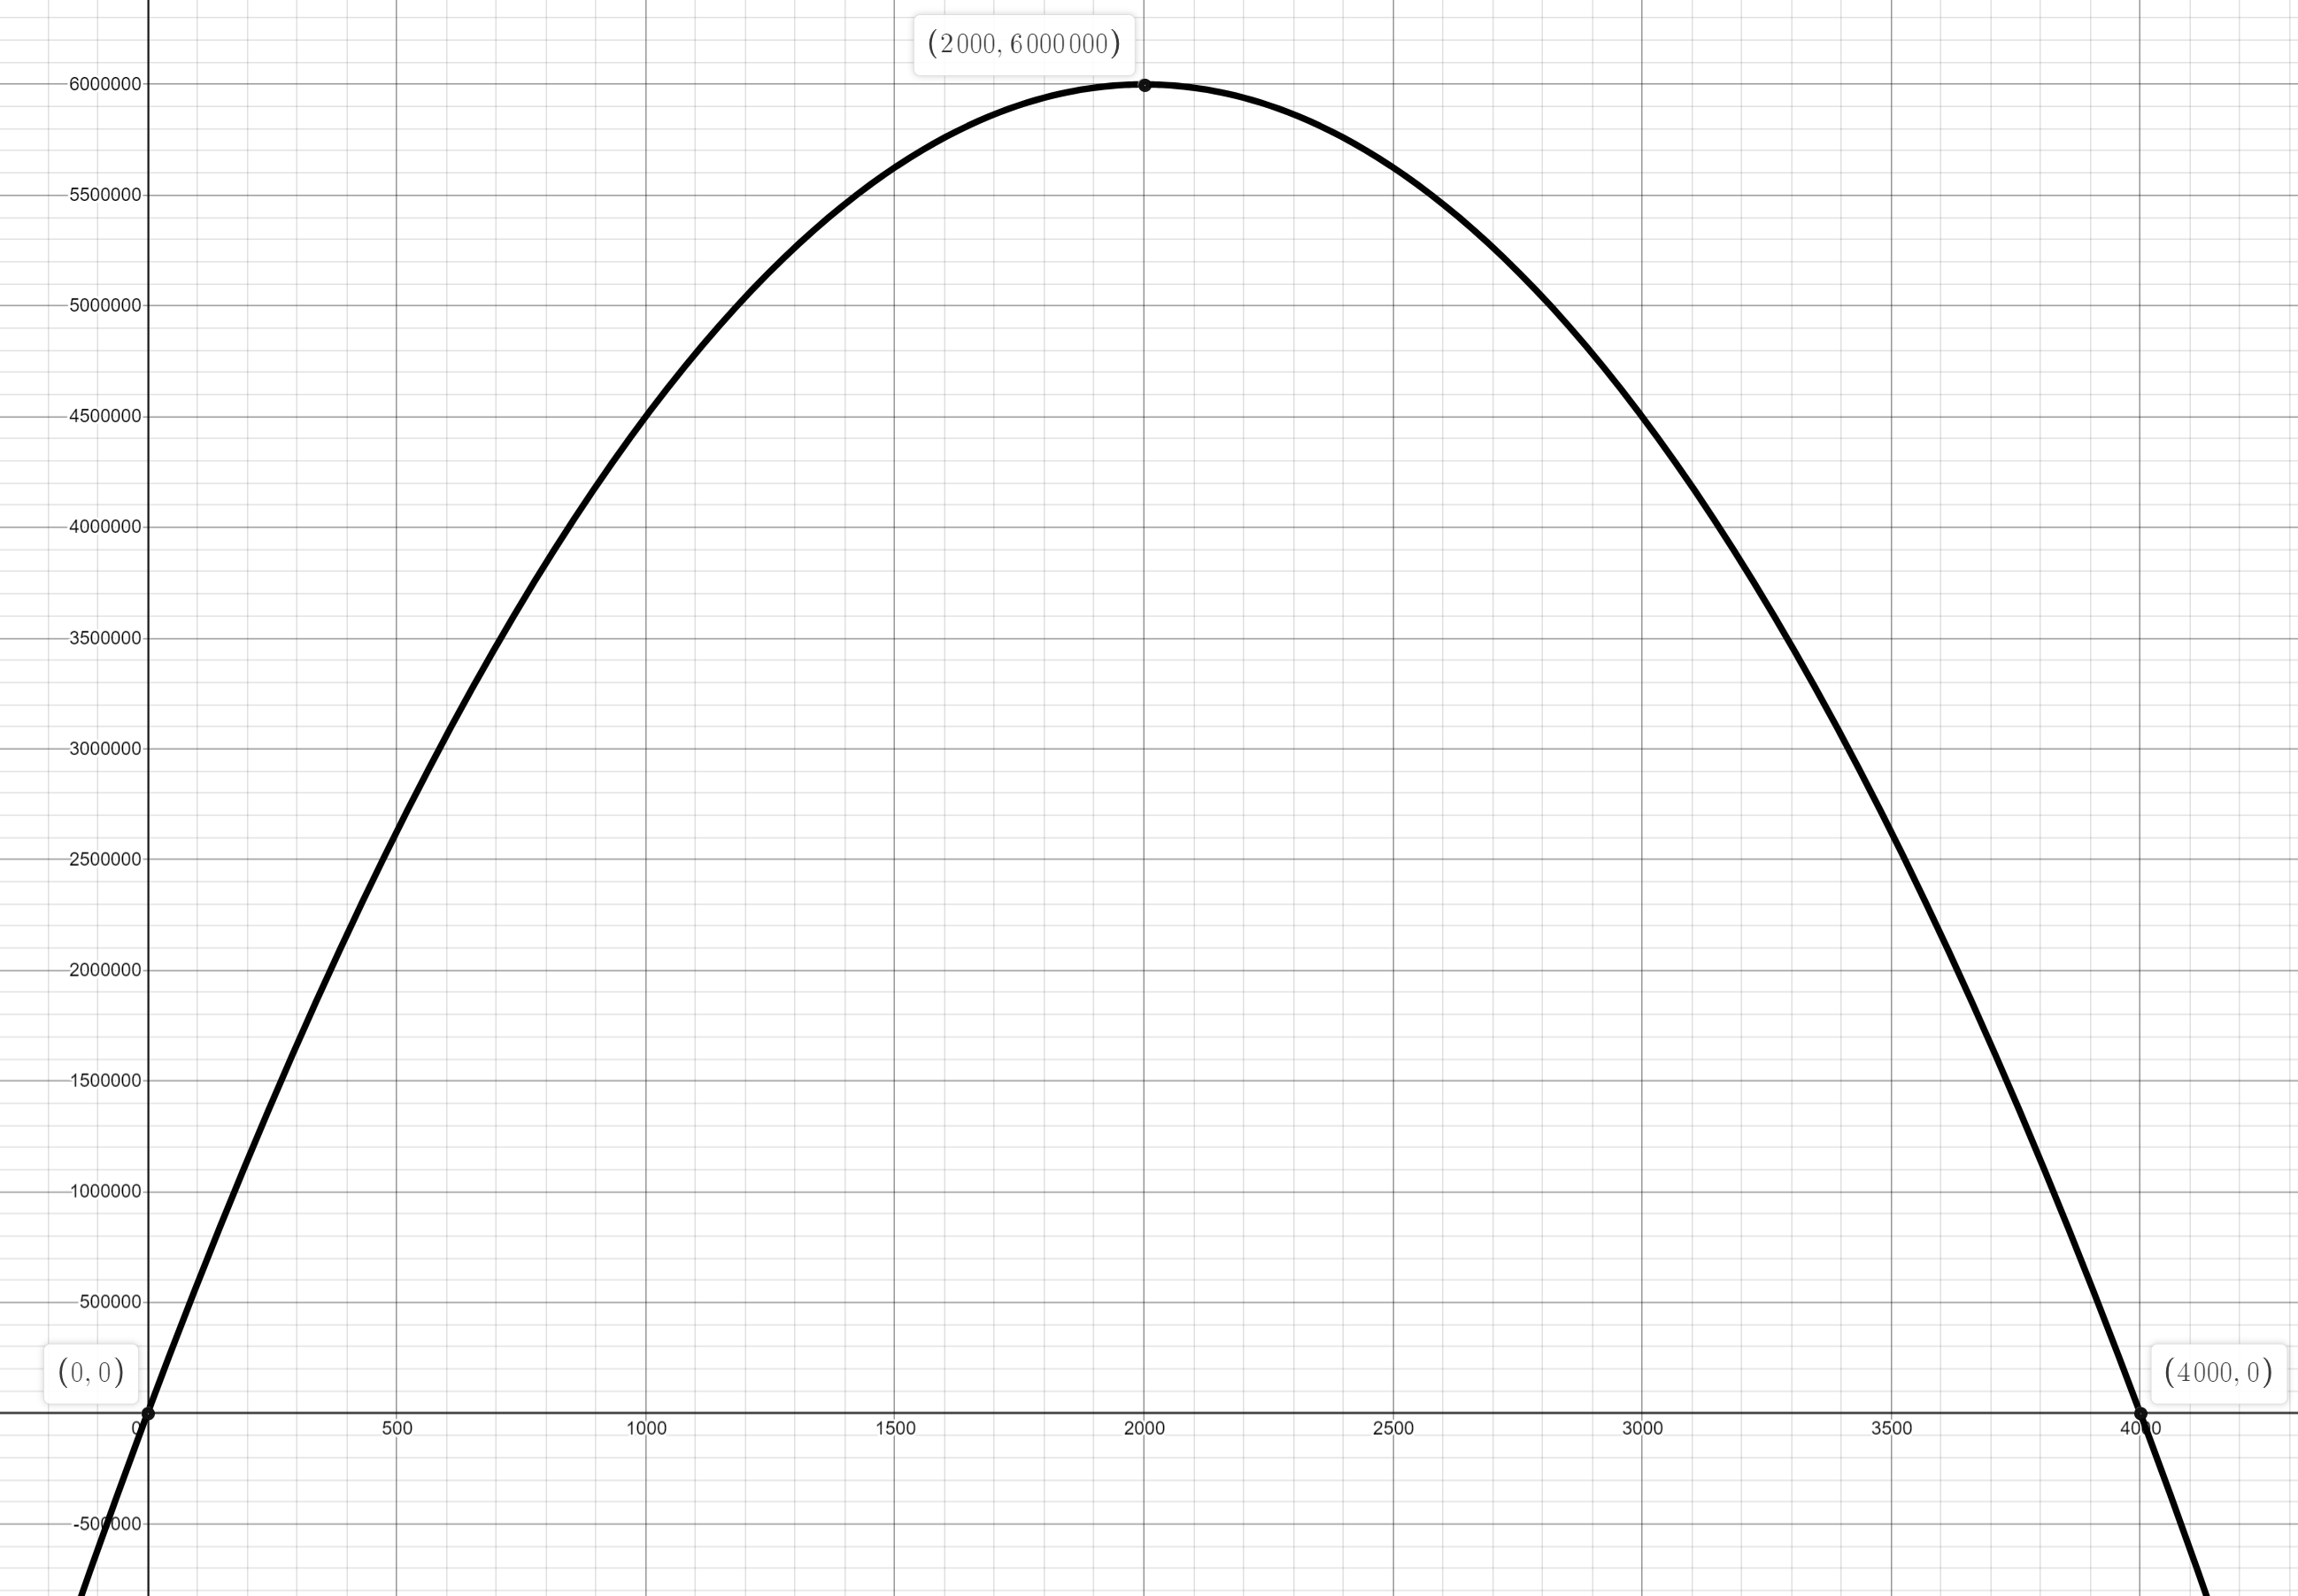
\includegraphics[scale=0.15]{images/appliedOptimization/Optimization_fencing2_ex10_4.PNG}
		%\caption{}
	    \end{figure}
    \end{minipage}
    
\end{multicols}


\newpage

%%%Example 1 from Calaway; 2.9; pg. 149%%%
\begin{example}
The manager of a garden store wants to build a 600 square foot rectangular enclosure on the store’s parking lot in order to display some equipment. Three sides of the enclosure will be built of redwood fencing, at a cost of \$7 per running foot. The fourth side will be built of cement blocks, at a cost of \$14 per running foot. 
\renewcommand{\labelenumi}{(\alph{enumi})}
\begin{enumerate}[leftmargin=*]

\item \textbf{Find the dimensions} of the \underline{least costly} such enclosure. Identify the \underline{objective equation} and the \underline{constraint equation}.
\item \textbf{Find the minimum cost} of the enclosure using the dimensions found in part (a).
\begin{figure}[h]
    \flushleft
    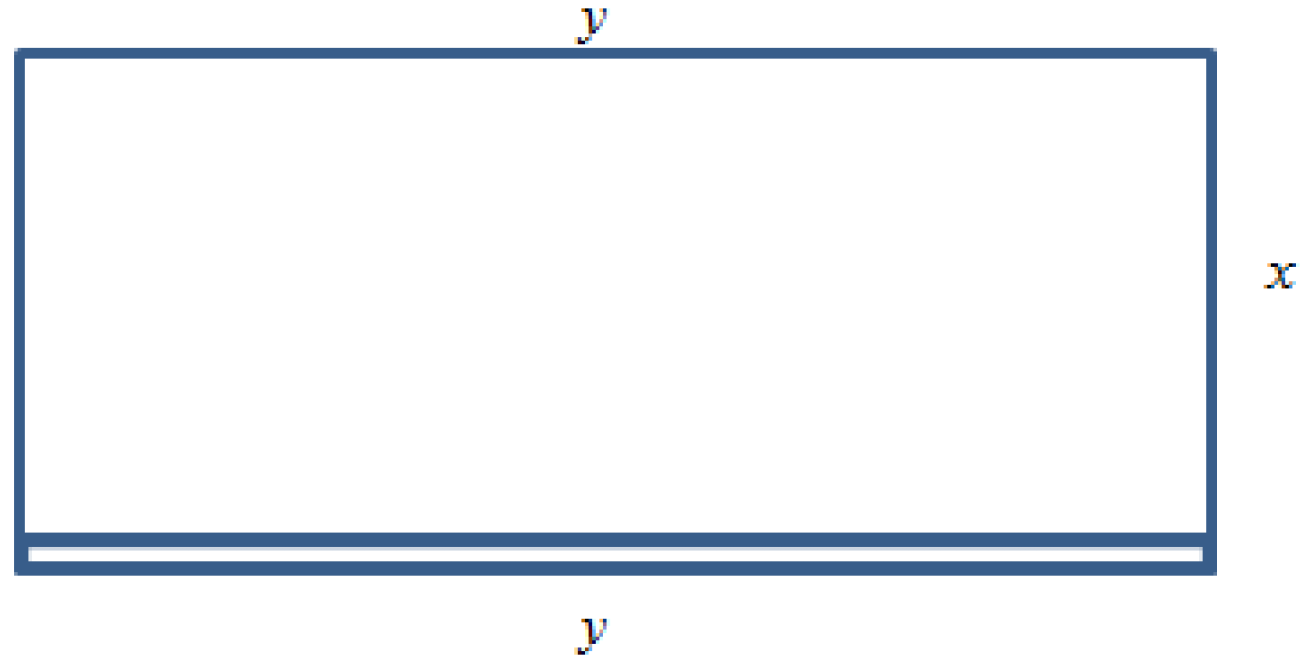
\includegraphics[width=0.4\textwidth]{images/optimization/exampleGardenStore.png}
\end{figure}

\end{enumerate}
    %%short answer
    
     \begin{sol}
    \begin{enumInline1}
     
     \item  $y=20$ feet; $x=30$ feet 
     \item  \$840 
  
    \end{enumInline1}
    \end{sol}
     
    %%solution
    \begin{solL}
    Complete solution here.....
    
    \end{solL}
    
\end{example}
\newpage





%%%%%%%%%%%%End Examples%%%%%%%%%%%%%%%%%%


%%%%%%%%%%%%%%%End Lesson%%%%%%%%%%%%%%%%%%
\Closesolutionfile{ans}
\Closesolutionfile{ansL}
\newpage
%%%Short Answers to Examples%%%
%\vspace*{\fill}
\subsection*{Short Answers to Examples}
%\vspace{-0.25cm}
%\begin{multicols}{2}
\input{ans9}
%\end{multicols}



